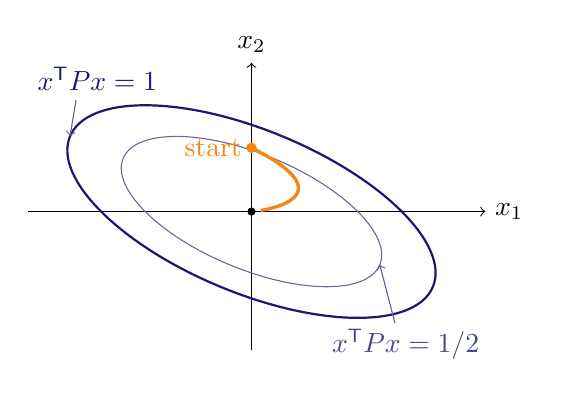
\begin{tikzpicture}[scale=1.35]
\draw[->] (-2.1,0)--(2.2,0) node[right] {$x_1$};
\draw[->] (0,-1.3)--(0,1.4) node[above] {$x_2$};
\draw[MidnightBlue,thick,rotate=-22.5] (0,0) ellipse (1.84776 and .76537);
\draw[MidnightBlue!65,rotate=-22.5] (0,0) ellipse (1.30656 and .54120);
\node[MidnightBlue] at (-1.45,1.25) {$x^{\mathsf T}Px=1$};
\draw[->,MidnightBlue!70] (-1.65,1.05)--(-1.7071,.7071);
\node[MidnightBlue!80] at (1.45,-1.25) {$x^{\mathsf T}Px=1/2$};
\draw[->,MidnightBlue!70] (1.35,-1.05)--(1.2071,-.5);
\draw[BurntOrange,very thick,domain=0:4,samples=90,variable=\t] plot ({1.2*\t*exp(-\t)},{.6*exp(-\t)});
\fill[BurntOrange] (0,.6) circle (1.4pt) node[left] {start};
\fill (0,0) circle (1.1pt);
\end{tikzpicture}
